% CS 410 Summer 2014 LaTeX template, based off of
% http://www.acm.org/sigs/publications/proceedings-templates

\documentclass{acm} % this finds the file "acm.bst"

\usepackage{cite,graphicx}

% this lets you include clickable URLs with \url{}
\usepackage[hidelinks]{hyperref}
\graphicspath{ {Images/} }

\begin{document}\sloppy % sloppy necessary here

\title{Sign Language Interpretation
    \titlenote{Submitted as the final project for CS 598 PS - Machine Learning For Signal Processing.}
}

\numberofauthors{3} % make sure you set this number
\author{%
    \alignauthor Saikat RoyChowdhury \\
    \affaddr{Dept. of Computer Science}\\
    \affaddr{University of Illinois at Urbana-Champaign}\\
    \email{rychwdh2@illinois.edu}
    \alignauthor Shyam Rajendran\\
    \affaddr{Dept. of Computer Science}\\
    \affaddr{University of Illinois at Urbana-Champaign}\\
    \email{srajend2@illinois.edu}
    \alignauthor Udit Mehrotra\\
    \affaddr{Dept. of Computer Science}\\
    \affaddr{University of Illinois at Urbana-Champaign}\\
    \email{umehrot2@illinois.edu}
}
\maketitle

\begin{abstract}
This work is part of a vision based American Sign Language Interpretation (ASL) system for natural human computer interface. It comes under the umbrella of much broader research field of hand gesture recognition. The aim of the paper is to develop a robust system which can interpret the American sign language digits from the static images, as well as video stream inputs. The system involves various important components like Hand segmentation from the background, wrist cropping, hand edge detection, extracting relevant features of the hand and a classifier for predicting the digit given the features. We also developed an algorithm for extracting the hand sign frames from a video input, which can then be used for classification. The final output of the system, predicts the digits shown in a video input and adds relevant subtitles to the video for the predicted digit at any given point during the video.
\end{abstract}

\keywords{Hand Segmentation, Wrist Cropping, Edge Detection, Largest Boundary Detection, Feature Extraction, Fourier Descriptors}

\section{Introduction}
Natural Human Computer Interaction is the demand of today's world. Among other body parts, hand gestures are the most natural and powerful communication modality for interaction with computer. In this project, we design and build a system which can recognize American Sign Language digits, from static images as well as video streams.\\
\\
There are two major approaches for Hand gesture recognition: Data glove and Vision based. The Data glove approach uses a glove with sensors attached to track finger blending, positioning and orientation. In this paper we have gone ahead with vision based approach, as it is more cost effective and feasible since the user does not have to wear a cumbersome device. In hand based gesture recognition systems, hand tracking and segmentation are the most important and challenging steps towards gesture recognition. Uncontrolled environment, lighting conditions, noisy background, skin color detection and rapid hand movements are some of the challenges that need to be considered while capturing and tracking the hand gestures.\\
\\
The second major step after Hand segmentation is Shape Feature extraction from the segmented hand. The shape feature extraction can usually be divided into contour based and region based. In our work, we have used contour based method which extracts shape feature information from the boundary of the entity. We have used Fourier descriptor method as it can overcome the effect of noise and boundary variations by analyzing the shape in spectral domain. Furthermore, they are compact, computationally light and there matching is a relatively simple process.\\
\\
The final step of the process involves training a classifier using the shape features extracted from the training data set collected, and using it to predict or classify a given gesture. In our work we have tried Neural Networks and K nearest neighbor algorithms for the purpose of classification, and have included the results obtained from each of the methods.\\
\\
To work with video inputs, we developed an algorithm for detecting the actual frames from the video where a digit is being shown and discard all the unnecessary frames where we are changing the sign from one digit to another. The system generates an \textit{SRT} file for the video, to show the predicted digits at relevant times during the video.\\
\\
In the following section we will discuss the various steps involved in hand segmentation in detail, which will be followed by feature extraction and classification in the later sections.

\section{Hand Segmentation}
When it comes to digit sign language recognition,  the prime area where most of the information is contained in the palm and fingers. So in order to maximize accuracy, the input data needs to be preprocessed, so that we clip out all the unnecessary or insignificant portions of the hand. Thus the primary step of hand detection is the skin color detection to segment the hand from the background. We used a well-known formulation to identify skin pixels[1][2].  A pixel is classified as a skin pixel if it satisfies an OR condition of the following formulas in RGB space and YCbCr space.
\begin{multline}
\begin{align}
    R > 95\quad \&\quad G > 40\quad \&\quad B > 20 \quad \&\\
    Max\{R,G,B\} - Min\{R,G,B\} > 15\quad \& \\
    |R - G| > 15\quad \&\quad R > G\quad \&\quad R > B
\end{align}
\end{multline}
\begin{multline}
\begin{align}
    Y = 0.299R + 0.587G + 0.114B\\
    Cr = 128 + 0.5R - 0.418G - 0.081B\\
    Cb = 128 - 0.168R - 0.331G + 0.5B\\
    85 < Cb < 135\quad \&\quad 135 < Cr < 180\quad \&\\
    Y > 80
\end{align}
\end{multline}
The OR condition is taken to account for variation of human skin colors and maximize segmentation accuracy. Thus the segmentation output is a matrix of 1's and 0's where 1 indicates something similar to skin color.

\begin{figure}[h]
\centering
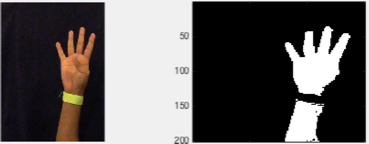
\includegraphics[width=3 in]{basic_black_background}
\caption{Segmentation with basic black background}
\label{fig:fig1}
\end{figure}

\begin{figure}[h]
\centering
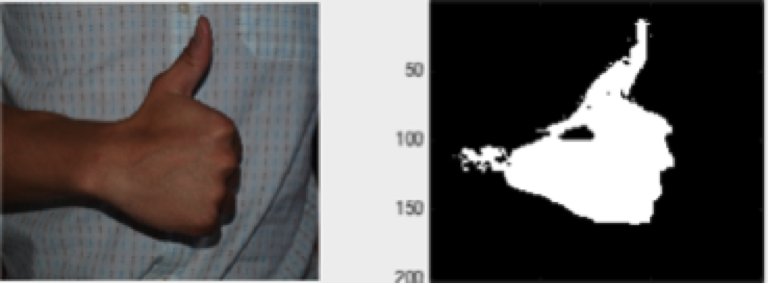
\includegraphics[width=3 in]{basic_colored_background1}
\caption{Segmentation with colored background}
\label{fig:fig2}
\end{figure}

\begin{figure}[h]
\centering
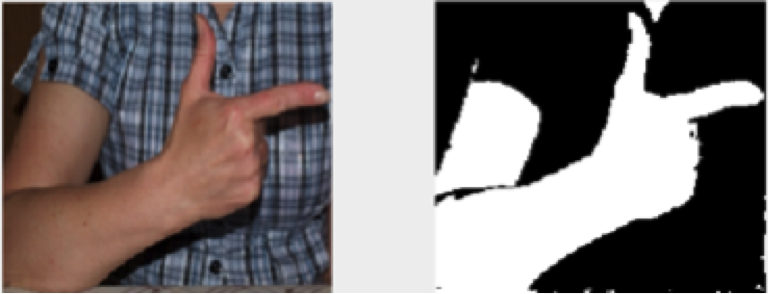
\includegraphics[width=3 in]{basic_colored_background2}
\caption{Segmentation with colored background}
\label{fig:fig3}
\end{figure}

\begin{figure}[h]
\centering
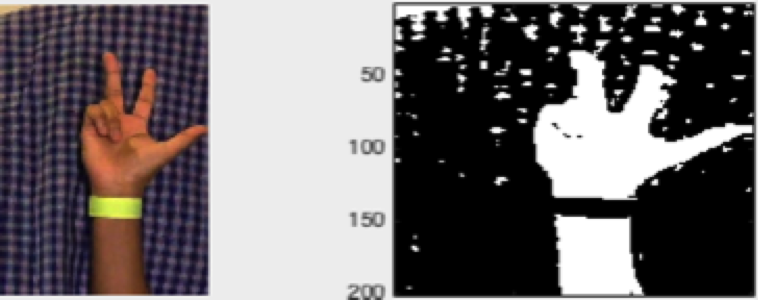
\includegraphics[width=3 in]{skin_colored_background}
\caption{Segmentation with some skin colored pixels in background}
\label{fig:fig4}
\end{figure}

\section{Hand Smoothening}
In order to minimize segmentation output, and additional step of smoothening is done. This involves passing the segmentation output through a median filter and a set of morphological operation. We used 2-D  median filtering technique, where each pixel is  the median of  n X n  neighborhood. On experimentation, we found that range of n=[4, 7] works well.  The next step of smoothing is using morphological close operation using two basic functions dilation and erosion. In dilation operation, the value of the output pixel is the maximum value of all the pixels in the input pixel's neighborhood. In a binary image, if any of the pixels is set to the value 1, the output pixel is set to 1. In Erosion operation, the value of the output pixel is the minimum value of all the pixels in the input pixel's neighborhood. In a binary image, if any of the pixels is set to 0, the output pixel is set to 0. We used matlab's \textit{imclose} function to achieve this effect.

\begin{figure}[h]
\centering
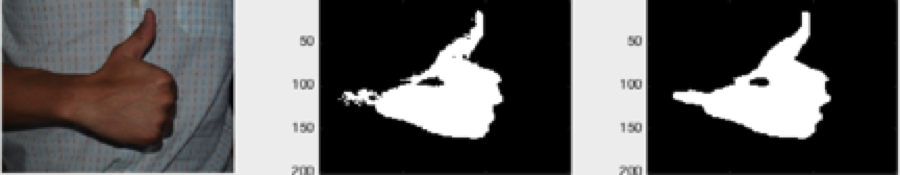
\includegraphics[width=3 in]{smoothening1}
\caption{Median filter and morphological close operations}
\label{fig:fig5}
\end{figure}

\begin{figure}[h]
\centering
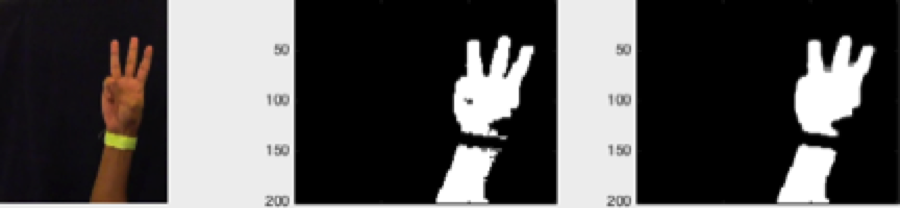
\includegraphics[width=3 in]{smoothening2}
\caption{Median filter and morphological close operations}
\label{fig:fig6}
\end{figure}

\section{Wrist Cropping}
Two classical approaches to detect wrist are width based and contour based detection [4][5][6]. In order to support random angle of  tilt of hand, then wrist detection becomes computationally intensive as it requires performing  4 way scans to identify in which direction the hand is pointing.  Another idea that we encountered is to use a principle component analysis based method to find the orientation method. However on performing experiments we found the applying PCA directly on the entire hand is not sufficiently accurate. An alternative method of making the user wear a wristband and detecting the principal component of orientation of the wrist-band gives much better result. The method is cost effective and completely removes all the compute heavy 4 way scans to detect hand orientation, and highly accurate. We detect the wrist-band, find its principal orientation 'x'(say), then the arm is orthogonal to the wrist band at (x+/- 90). Thus we make the hand rotation invariant and then use a simple width based wrist detection algorithm to clip the forearm below the wrist.

\textit{Width based wrist cropping} - Since the segmented hand is rotation normalized now, we use a simplified width based wrist cropping algorithm. We scan from image from bottom to top row, and calculate the number of hand pixels in each row and form a distance vector. We then use a smoothing filter to distance vector plot. The next step is to find min peak that gives the row position where we need to crop the image.
Another alternative approach can be to find the top most row where we can locate a wrist band color pixel and clip all the rows below that. We do not see any significant performance gain and width based cropping gives a better result.
\begin{figure}[h]
\centering
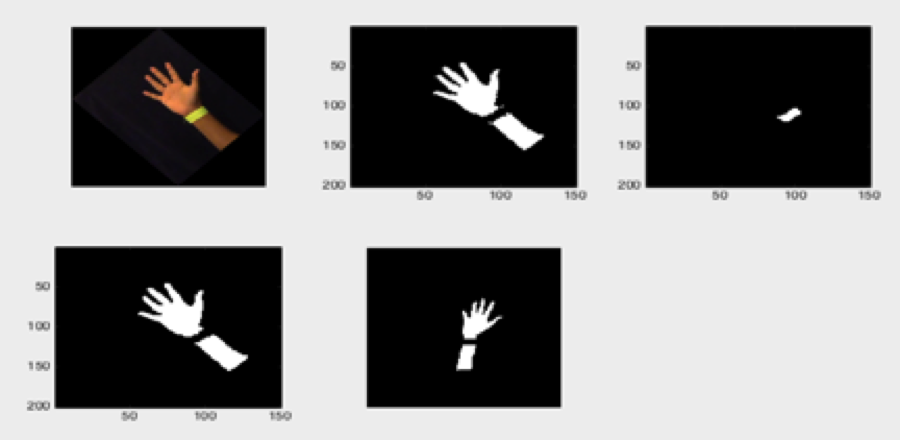
\includegraphics[width=3 in]{wrist_cropping1}
\caption{Wrist Cropping}
\label{fig:fig7}
\end{figure}

\begin{figure}[h]
\centering
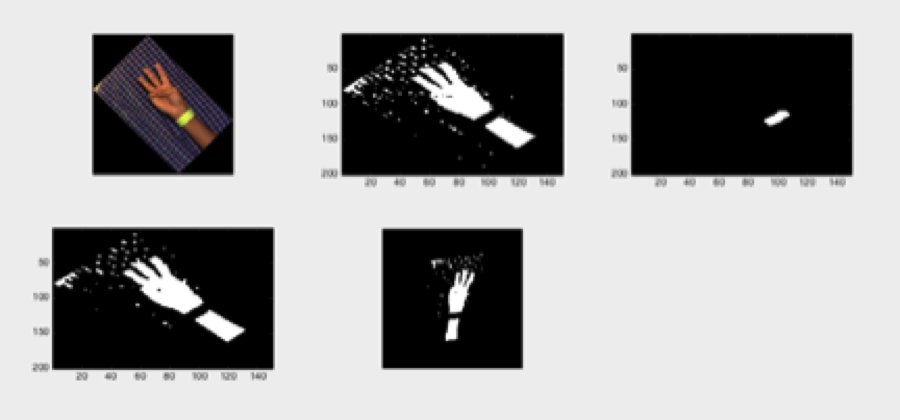
\includegraphics[width=3 in]{wrist_cropping2}
\caption{Wrist Cropping}
\label{fig:fig8}
\end{figure}
Figure 7 and 8 - From top to bottom in clockwise (1) Original tilted hand (2) skin color based segmentation  (3) Wrist band Detection and PCA for orientation detection (4) image smoothing using median filter/morphological close (5) Rotation normalized image

\section{Edge Detection}
Now that we have a wrist cropped hand, we are a step closer to extraction shape feature descriptor. We perform well known Canny Edge detection algorithm [8] to outline the contour of the hand gesture. The basic steps of the edge detector involves:
\begin{enumerate}
\item Apply Gaussian filter to smoothen the noise
\item Find intensity gradients of the image
\item Apply non-maximum suppression to get rid of spurious response
\item Apply double threshold to determine potential edges
\item Use a hysteresis based approach to track edges and suppress weak edges
\end{enumerate}

\section{Largest Boundary Detection}
In order to counter spurious background objects which did not get filtered out in the skin detection stage, because those objects had similar color to hand pixels, we perform Moore-Neighbourhood tracing algorithm [8] [9], to detect the boundaries and select the biggest boundary. We have used matlab \textit{bwboundaries} function for this algorithm. This works on the assumption that the palm and fingers form the biggest boundary, which is true most of the time. Such a method helps us in eliminating and skin color background objects (like a distant face etc).
\begin{figure}[h]
\centering
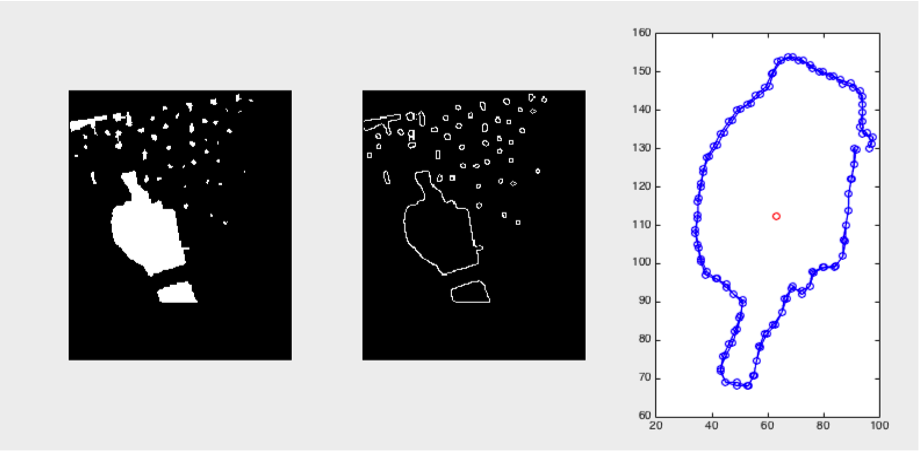
\includegraphics[width=3 in]{largest_boundary1}
\caption{Edge and largest boundary detection}
\label{fig:fig9}
\end{figure}

\begin{figure}[h]
\centering
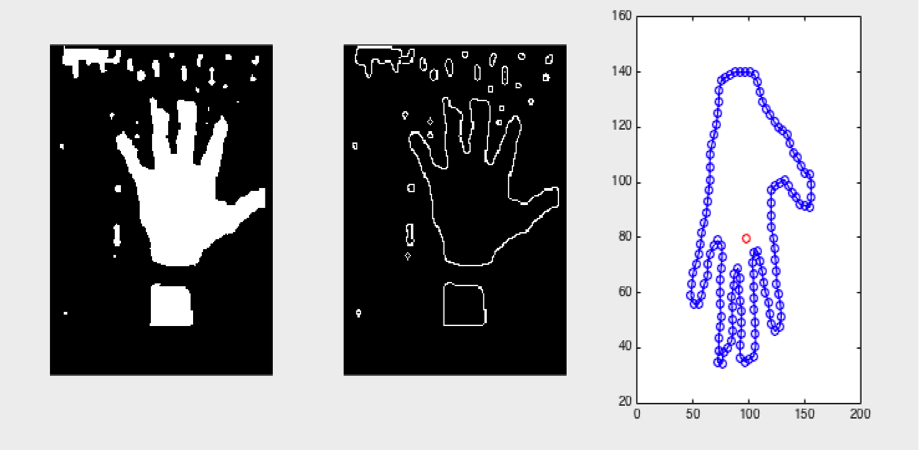
\includegraphics[width=3 in]{largest_boundary2}
\caption{Edge and largest boundary detection}
\label{fig:fig10}
\end{figure}

\begin{figure}[h]
\centering
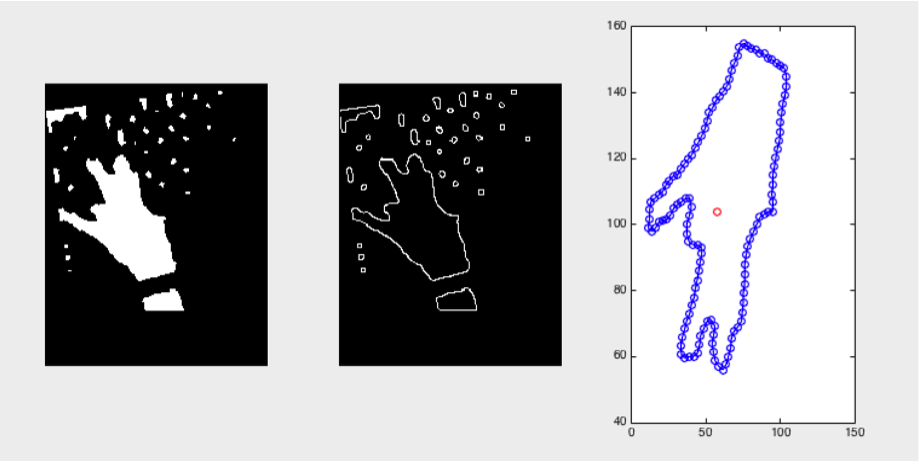
\includegraphics[width=3 in]{largest_boundary3}
\caption{Edge and largest boundary detection}
\label{fig:fig11}
\end{figure}

Figure 9, 10, 11 - From left to right (1) segmented hand based on skin color (2) edge detector output (3) Select the largest boundary using Moore-Neighbourhood Algorithm and arc-tan sampled points of the boundary

\section{Feature Extraction}
Feature extraction refers to the process of extracting features the hand segment processed in the previous step. For our purpose we have used Contour based feature extraction, which extracts shape information from the boundary of the hand segment in the image provided. We used Fourier descriptors which is one of the most widely used method for contour based shape feature extraction. The method uses shape boundary coordinates to compute Shape signature functions which can then be analyzed in the frequency domain.\\
\\
We first compute the boundary pixels of the hand using the Canny edge detector to get the pixel set:
$$P = {(x(t) , y(t)) | t \epsilon [1 N]}$$
Since hand segments boundary size will be different, we have to sample the boundary pixels to have same number of boundary points. This further smooths down the boundary detected. We explored two sampling methods, namely \textit{Equal Points Sampling} and \textit{Equal Arc Length Sampling}. Equal points sampling selects points spaced at equal number of points along the shape boundary. The equal arc length sampling selects points spaced at equal arc length along the shape boundary. So we select 64 candidate points using the above sampling methods. We chose a power of 2 for the number of points, so as to facilitate the use of Fast Fourier Transform. Arc length sampling is what we finally went ahead with, as it was giving much better results.\\
\\
After normalization, we compute the Shape signature function which is a 1-D function representing 2D areas or boundaries. We considered two signature functions: Centroid distance and Complex coordinates.
\begin{itemize}
\item Complex coordinates : Complex number generated from boundary coordinates $$z(t) = x(t) + iy(t)$$ To eliminate the effect of bias, the coordinates are shifted by subtracting the centroid i.e $$z(t) = [x(t) - x_c] + i[y(t) - y_c]$$ where $(x_c,y_c)$ is the centroid of the shape. This shift makes the shape invariant to translation.
\item Centroid distance : It is expressed as the distance of the boundary points, from the centroid $(x_c, y_c)$ of the shape $$r(t) = ([x(t) - x_c]^{2} + [y(t) - y_c]^{2})^{1/2}$$
For a given shape signature, which is normalized to 64 points we compute the Discrete Fourier Transform to get the coefficients which are called Fourier Descriptors. We make the Fourier descriptors Rotation invariant by ignoring the phase information and by taking only the magnitudes of the descriptors. For the complex coordinates signature, all except the first descriptor is required to index the shape. 
\hfill \break
\hfill \break
We achieve scale normalization, by dividing the magnitude of all the other descriptors by the magnitude of the first descriptor. For the centroid distance signature there are only N/2 different frequencies and so only half the Fourier descriptors are needed to index the shape.

\end{itemize}

\section{Classification}
\subsection{K nearest neighbor}
As a first step, after feature extraction we tried the k nearest neighbour classification algorithm to predict the hand gestures. We trained the classifier on nearly 1600 hand samples of American Sign Language digits, with various types of backgrounds and experimented with various values of k. Here is a plot of how the classifier performed on the training data set itself:
\begin{figure}[h]
\centering
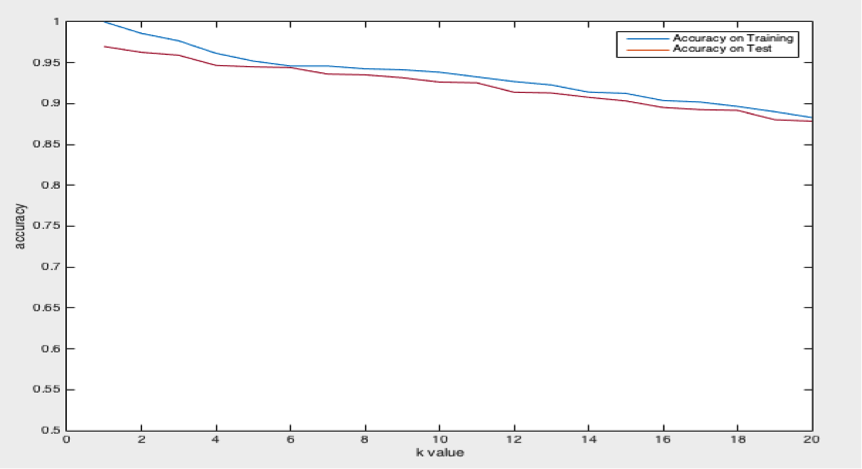
\includegraphics[width=3 in]{knn}
\caption{K nearest neighbour Accuracy Plot}
\label{fig:fig12}
\end{figure}
\\
For the purpose of our experiment, we divide our dataset consisting of around 2200 samples of ASL digits randomly, and use 70\% of it for training and the remaining 30\% for testing. From the above plot we see that we get the highest accuracy of 100\% on training set and 95\% on the test set for when the value of k is 1 (nearest neighbour). As we go on increasing the value of k, we observe a decrease in the accuracy value. On an average we get an accuracy of around 50  - 55\% on a random test data set, with the highest accuracy recorded of 65\%.
\subsection{Neural Networks}
We used a feed forward neural network with sigmoid transfer functions for hidden and output layer neurons to train the network to recognise hand gesture. Backpropagation algorithm is used to learn the weights and biases for the neurons. 

\begin{figure}[h]
\centering
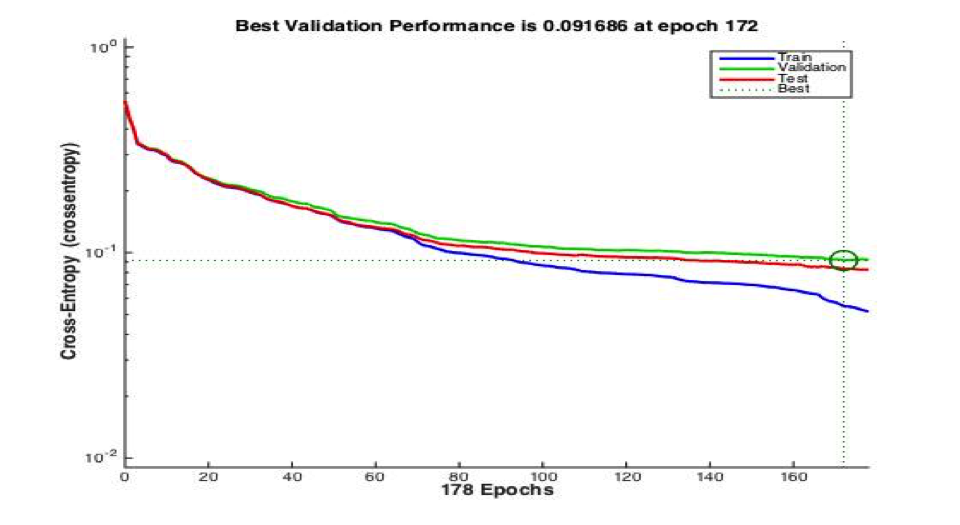
\includegraphics[width=3 in]{nn_error_plot}
\caption{Neural Networks Error Plot}
\label{fig:fig13}
\end{figure}

The neural network contains 64 input nodes (since we have 64 point Fourier Descriptors features per digit), 'N' hidden neurons and 11 output neurons(digits 0 to 10). We experimented with varying numbers of hidden layer neurons. For N = 48, the network was able to learn the shapes with reliable accuracy. We collected multiple hand gestures for each digit for every team member. Around 1600 samples of digits were used to train and test the system. We used \textit{Matlab Neural Network Toolbox} to construct and train the network. 


\begin{figure}[h]
\centering
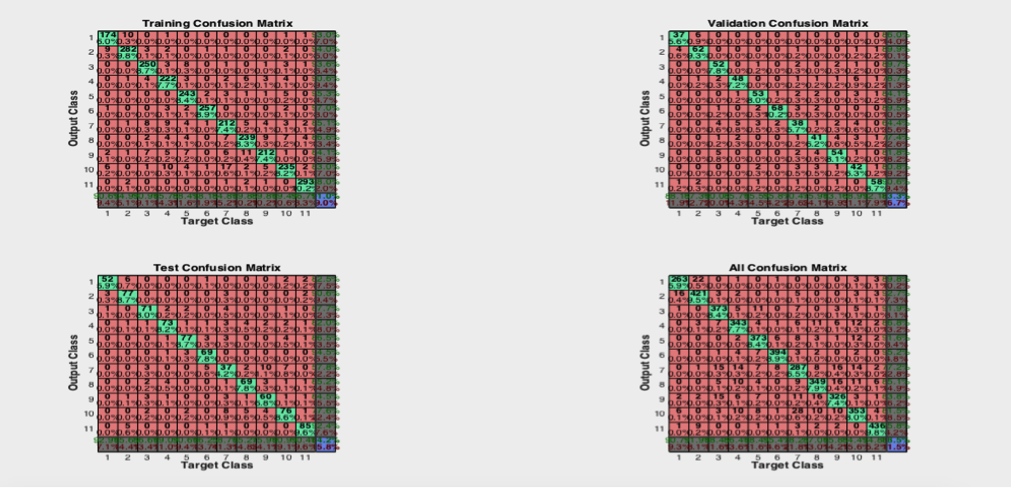
\includegraphics[width=3 in]{nn_confusion_matrix}
\caption{Neural Networks Confusion Matrix}
\label{fig:fig14}
\end{figure}


We divided the dataset into 65-70\% for training, 15\% for validation and 15-20\% for testing. Validation dataset helped in fine-tuning the network so that it doesn't overfit to training samples. Overall we see highest accuracy of around 84\% on the testing set, 91\% on the training set and 83\% on the validation set as shown in the confusion matrix below. On average we see accuracy of around 70-80\% on random test samples.


\section{Recognition from continuous video}
\subsection{Detecting the transition peaks}
The main challenge in gesture recognition is that the gesture transitions are continuous and not discrete. The demarcation unit between the different frames need to be computed programmatically. Two approaches were tried out for this purpose. The initial idea was to find the XOR relation or frame difference between the frames to detect changes during the gesture transition. The video file is analyzed frame by frame and the differences in successive frames are computed to a RMS value. The plot of RMS values is shown as below in figure 13.

\begin{figure}[h]
\centering
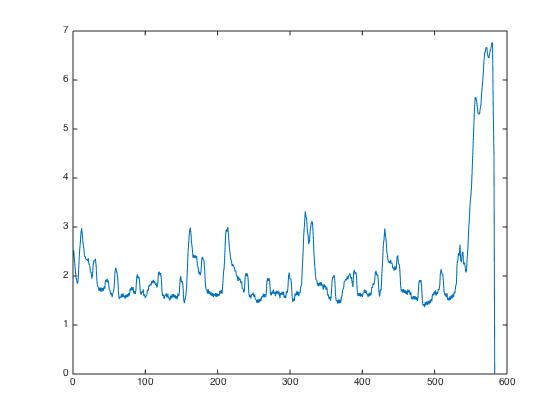
\includegraphics[width=3 in]{peaks1}
\caption{Gesture Transition Plot}
\label{fig:fig15}
\end{figure}


The frame difference plot is then smoothened and passed through a peak finder algorithm that detects the peaks on the plot. The the indices of the the peaks that correspond to the frame number of the video and the corresponding timestamp, calculated based on the frame rate of the video, provides the set of frames where the gesture transition occurred as in figure 14.

\begin{figure}[h]
\centering
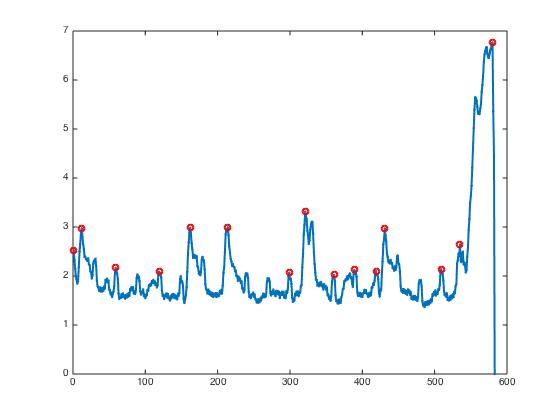
\includegraphics[width=3 in]{peaks2}
\caption{Peak Plot corresponding to the and signs}
\label{fig:fig16}
\end{figure}
\\
We also consider a set of frames post the peak, that indicate the gesture hold frames and include them to the test frames.  These set of test frames are fed into the Neural Network working on Fourier Descriptor algorithm that predicts the related class of the gesture ( one for each digit in the American Sign Language ).  The predicted set is time synced against the corresponding frame in the video and a .srt subtitle is generated. Window prediction for gesture hold frames. The set of gesture hold frames might produce different class predictions. The window majority is considered for the duration of start to end frame within the window and this is used in the .srt for the duration of the video window. 

\begin{figure}[h]
\centering
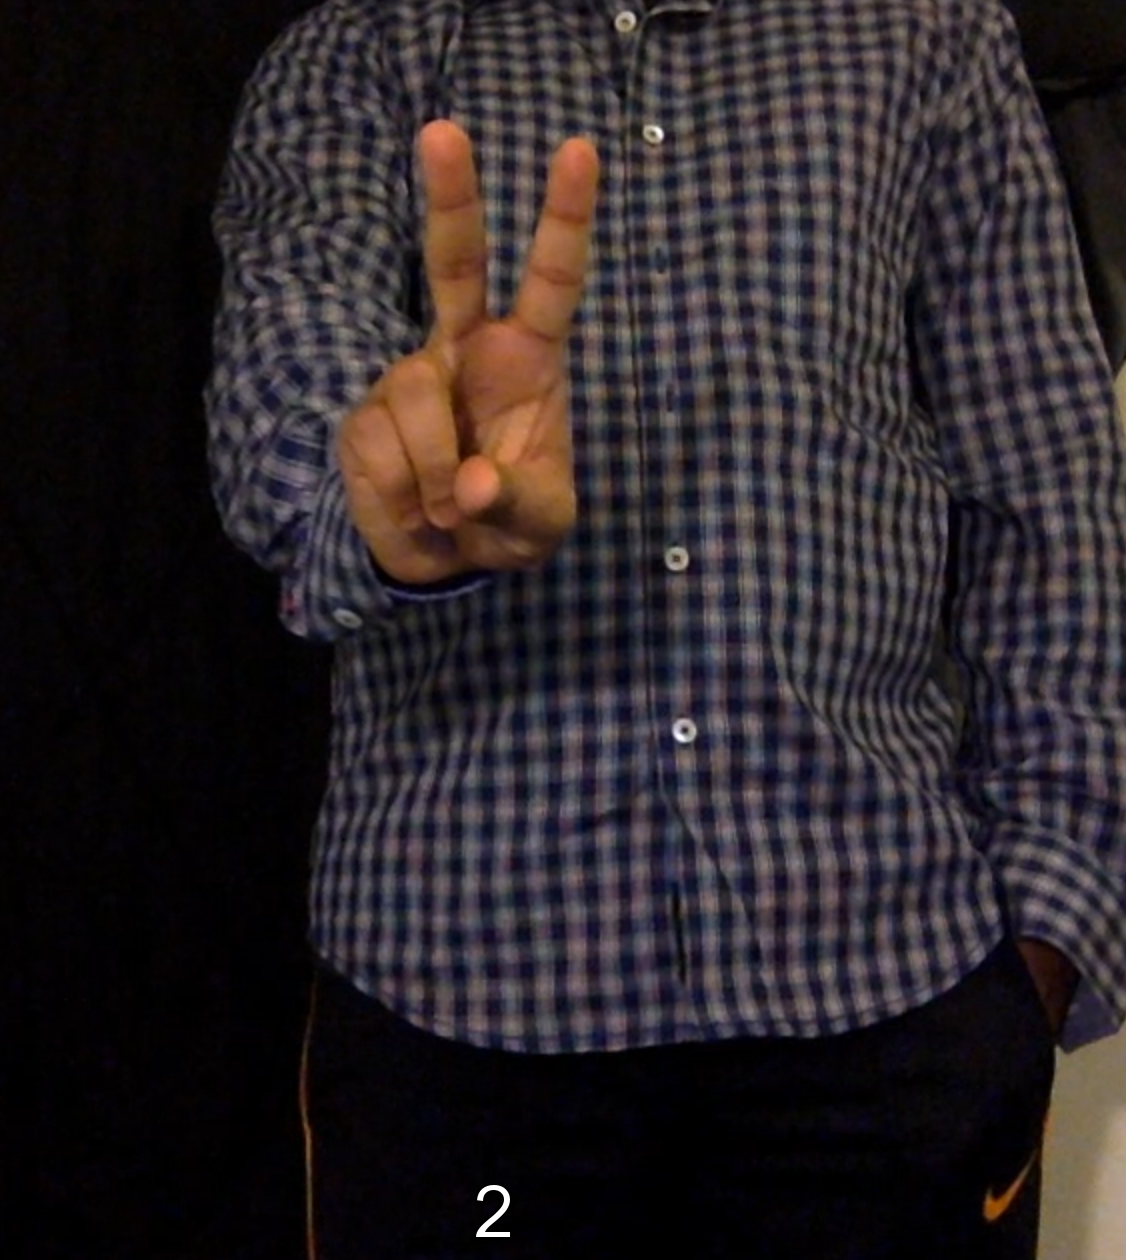
\includegraphics[width=1 in]{2}
\caption{}
\end{figure}


\begin{figure}[h]
\centering
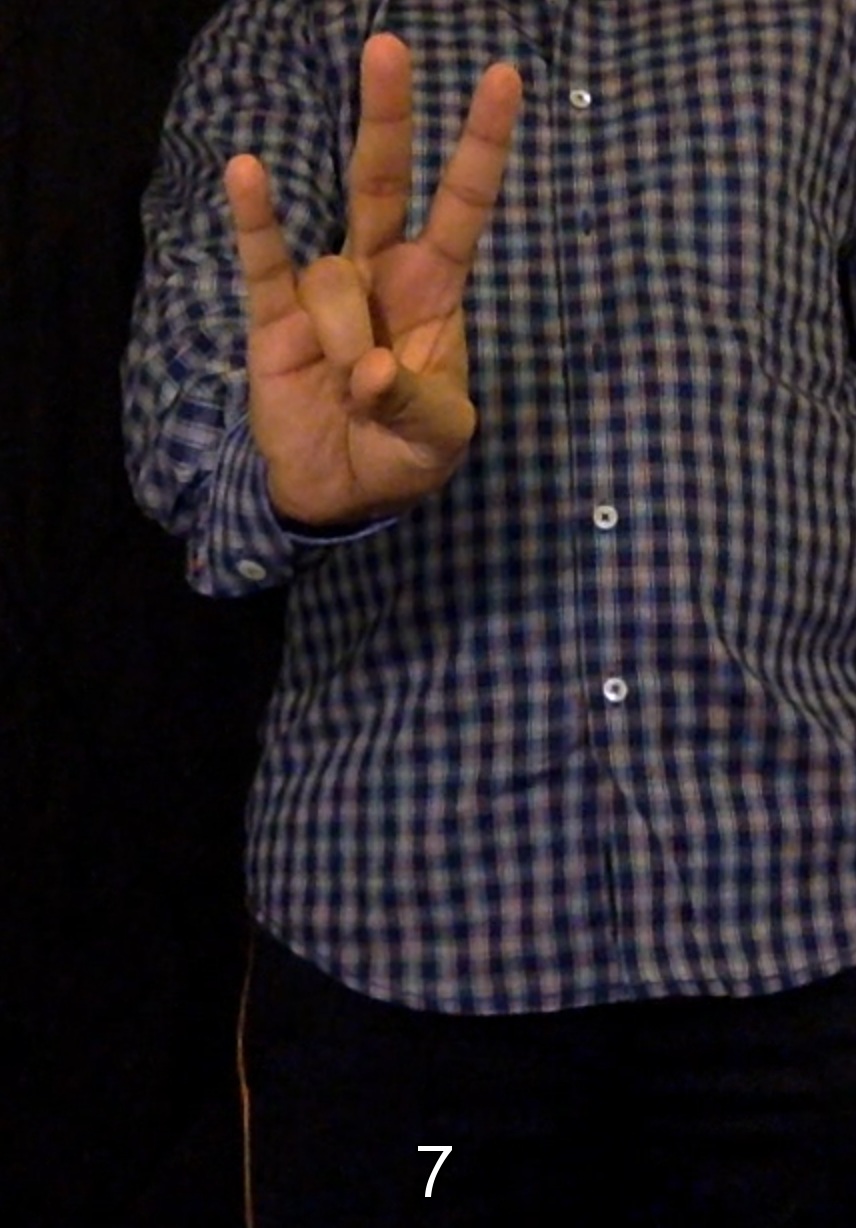
\includegraphics[width=1 in]{7}
\caption{Below is a screen grab of video subtitle generated by taking mode of the predicted classes within a set window of images}
\label{fig:fig18}
\end{figure}


\bibliographystyle{plain}
\bibliography{bib} % "bib" is the name of the .bib file


\end{document}
